\documentclass{jabstract}

\jtitle{インドネシアにおける2025年軍事法案を巡る世論に関するX(旧Twitter)上の感情分析}
\jauthor{クリスティアン ハルジュノ}
\jaffiliation{情報工学分野}
\jteacher{本間宏利}

\begin{document}
\maketitle

\begin{multicols}{2}
  
\section{はじめに}
インドネシア国軍法案 (別名 Rancangan Undang-Undang Tentara Nasional Indonesia または RUU TNI)の改正は, 2025年3月20日に法として成立した際, 大きな論争を巻き起こした. 主な論点は特に第47条にあり, この条文は (武器を携帯する権利を持つ)現役軍人が非防衛分野の文民職に任命されることを規定しており, これは1998年以降の民主化改革を覆すものである. これは, 軍の二重機能 (Dwifungsi ABRIとしても知られる)\cite{HRW2024}の復活に関する重大な懸念を引き起こす. 本研究はインドネシアのソーシャルメディアのパラダイム, より具体的には, インドネシア全国の市民にとって公平な議論の場として機能したX (旧Twitter)に焦点を当てる. \#TolakRUUTNIなどのハッシュタグが, インドネシア政府への抗議の一形態として大規模に使用された\cite{CNN2024}.

本研究は, X上での公開された言説の感情分析を行うことにより, RUU TNI 2025に対する国民感情を定量化し分析することを目的とする. 具体的な目的は, 法案が最初に提案された時から正式に署名された後の数ヶ月間にわたる感情の極性の分布を測定し, 国民の不満の主な要因を特定することである. この分析は, Xの検索エンジンから取得した20万件以上のツイートからなるコーパスを使用する.
\section{先行研究}
The sentiment analysis of social media data, particularly regarding this specific legislative issue in Indoensia has been extensively studied with degrees of success and different methodical approaches. 

\subsection{サブセクション}
必要に応じてサブセクションを設ける。しかし、紙面も限られているので本当
にサブセクションが必要かどうかは、今一度考えてみるといいだろう。サブセ
クションにせずとも、適切に段落分けすることで、十分読みやすい文章にする
ことが可能な場合が多いはずだ。
表(表~\ref{tab:sample})や図(図~\ref{fig:sample})の使い方も重要になる。

\begin{tablehere}
  \noindent
  \parbox{\linewidth}{
    \centering
    \caption{表の挿入例}\label{tab:sample}
    \begin{tabular}{|c|c|c|}
      \hline
      & jarticle & jpreprint\\
      \hline
      一段に収まる図 & figure環境 & figurehere環境\\
      \hline
      紙幅一杯の図 & figure*環境 & figure*環境\\
      \hline
      一段に収まる表 & table環境 & tablehere環境\\
      \hline
      紙幅一杯の表 & table*環境 & table*環境\\
      \hline
    \end{tabular}
  }%
\end{tablehere}

\begin{figurehere}
  \noindent
  \parbox{\linewidth}{
    \centering
    \scalebox{0.5}{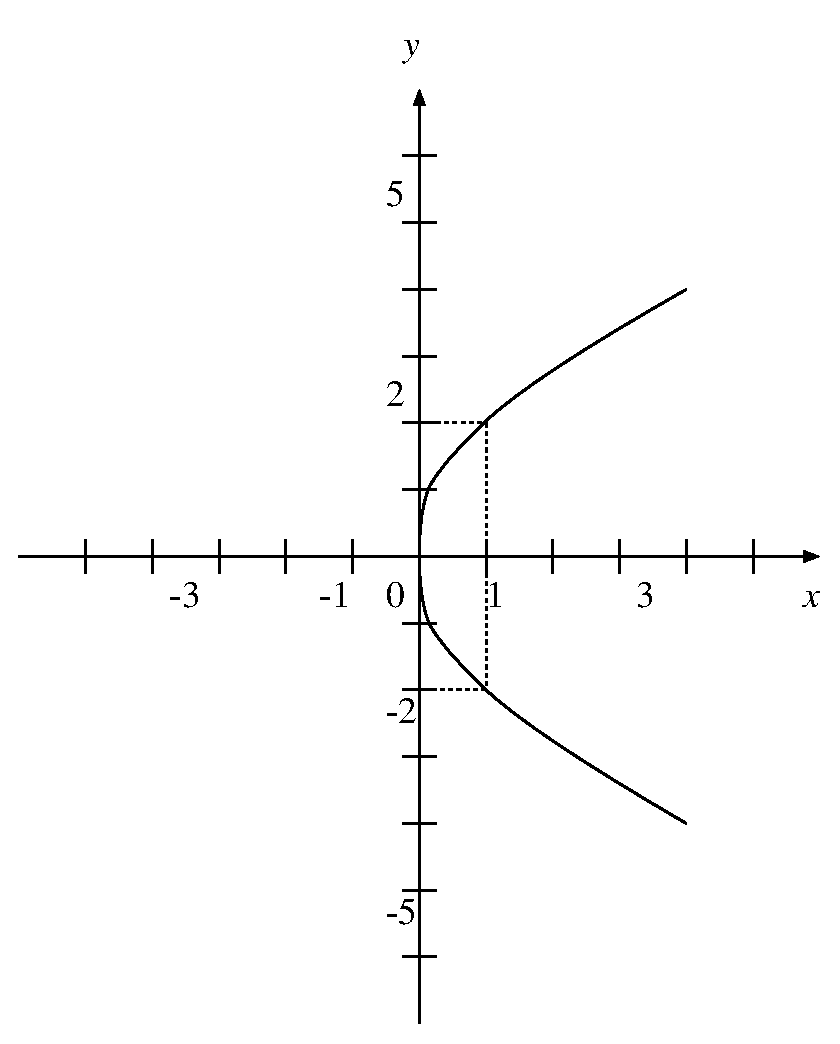
\includegraphics{sample.eps}}
    \caption{図の挿入例}\label{fig:sample}
  }%
\end{figurehere}

\section{次のセクション}
中間発表の場合は進捗状況や今後の方向性、進め方など、本発表の場合は自分
の研究の核心部分や実験などがこのあたりに来ることになるだろう。

\begin{enumerate}
\item あれ
\item これ
\item それ
\item どれ
\end{enumerate}
箇条書きは紙面を食うので、必要性を慎重に考えなければならない。

\section*{おわりに}
最後に全体をまとめ、自分の研究の成果と課題をはっきりさせることが肝心と
なる。文章全体の印象を左右することにもなるので、ここも気は抜けない。

{\small
\bibliographystyle{plain}
\bibliography{references.bib}
}

\end{multicols}

\end{document}
